\chapter{Antecedentes}
Durante este capítulo se describen las bases teóricas que sustentan este proyecto: Visión computacional y procesamiento de imagen y Planeación de movimientos. Se describen herramientas como segmentación por color, operaciones morfológicas, filtrado y detección de bordes, análisis de los movimientos de un manipulador, entre otras.

\section{Robots de Servicio en entornos Industriales}

Bajo la opinión de Babel en \cite{babel_industry_2022} La Industria 4.0 tiene como objetivo la \textit{interconexión directa e inteligente} de  personas, máquinas y productos. De acuerdo con el autor, esta \textit{interconexión inteligente} se refiere en este contexto a:
 \begin{itemize}
     \item Producción flexible
     \item Fábricas convertibles
     \item Soluciones enfocadas en el consumidor
     \item Logística optimizada
     \item Red de datos estandarizada
     \item Administración de reciclaje de recursos
     \item Digitalización de la producción
 \end{itemize}
 El autor también describe que bajo su perspectiva, la llamada Industria 4.0 consiste en la producción industrial en red y que busca optimizar la cadena de valor y mejorar la administración del ciclo de vida de las plantas y fábricas en la red global. La introducción de robots de servicio móviles que realicen actividades de apoyo dentro de las instalaciones de una fábrica pueden contribuir con estos dos últimos objetivos, colaborando en la transformación de las plantas hacia un modelo más flexible y permitiendo diversificar las actividades que se realizan en ellas.

Tradicionalmente, la robótica de servicio ha tenido como objetivo ser de ayuda para usuarios que por cualquier motivo se encuentren con dificultades para realizar tareas que sean repetitivas, sucias o incluso peligrosas, teniendo como foco aquellas actividades a realizar dentro de un entorno doméstico. En la actualidad, este tipo de robots aún se encuentran en constante desarrollo y no se cuenta todavía con una introducción real de estas herramientas en la cotidianeidad de las ciudades, siendo un poco más comunes en centros de desarrollo como universidades o institutos de investigación. Sin embargo, las habilidades mediante las cuales llevan a cabo las tareas que se menciona, son extrapolables y útiles fuera del ambiente doméstico. 

De acuerdo con la Federación Internacional de Robótica, se define un \textbf{robot de servicio profesional} como \textit{aquel que es utilizado en tareas comerciales, y para el cual se requiere cierto grado de autonomía, ya sea parcial o completa} \cite{ifr_international}. Los robots que se busca tratar en este documento cuentan con un grado alto de autonomía, partiendo de la idea de que, una vez asignada una tarea y con el conocimiento previo que se considera necesario, el robot debe ser capaz de llevar dicha tarea a término, siendo idealmente resistente a cambios en las condiciones del entorno.
  
\section{Visión Computacional}
La visión es una de las herramientas básicas con la que la mayoría de los seres vivos cuenta, es un proceso que realizamos día a día sin que nos represente un gran esfuerzo y a través de ella somos capaces de distinguir formas, profundidades, colores, entre otras características de los objetos de forma automática, realizando complicados cálculos y análisis sin ser conscientes de ello. Es por este motivo que utilizar sistemas para aprovechar la información disponible mediante el análisis computacional de imágenes es una temática que se encuentra con frecuencia entre las investigaciones desde hace décadas. Uno de los ejemplos más representativos de esto es la obra póstuma \textit{Visión}, del científico cognitivo David Marr (1945-1980) publicada en 1982. En este trabajo, Marr propone los siguientes tres niveles en los cuales descompone la percepción visual humana:

\begin{itemize} 
    \item \textbf{Computacional}: en el cual se determina aquello que se busca estudiar.\\
    \textit{¿Qué tarea se realiza?}
    \item \textbf{Representación y algoritmo}: donde se plantea la representación que se le dará a las entradas y salidas, además del algoritmo que se utilizará para su procesamiento, es decir, la forma en que el sistema cognitivo realiza la actividad \\
    \textit{¿Cómo se lleva a cabo la tarea?}
    \item \textbf{Implementación en hardware}, corresponde al mecanismo físico que se ha de usar para obtener las representaciones y ejecutar el algoritmo seleccionados en el nivel anterior \\
    \textit{¿Qué dispositivo puede realizar la tarea?}\cite{freire_importancia_2007}
\end{itemize}

El autor Richard Szeliski \cite{szeliski_computer_2022}, menciona que el objetivo de la visión computacional es describir el mundo que vemos en una o más imágenes y reconstruir sus propiedades (forma, iluminación o distribución de colores). Simulando así una forma de imitar el comportamiento de la visión de los seres vivos, mediante máquinas y algoritmos computacionales. Haciendo una relación con la teoría de Marr, los dos primeros niveles son conceptualmente similares. El tercer nivel, el de la implementación, es el que encuentra el mayor cambio, reemplazando a los agentes biológicos por equipos de cómputo que puedan otorgar la información necesaria para extraer la misma información de las imágenes que obtendría el sistema de visión humano.


Afortunadamente, la visión computacional se encuentra en constante desarrollo, tanto en cuestión de hardware como en relación a los algoritmos que se utilizan, y su uso se encuentra presente en gran variedad de aplicaciones.


El elemento base de este análisis es la \textbf{Imagen}. En \cite{gonzalez_digital_2002} González y Woods la definen como una función bidimensional $f(i,j)$, donde $i$ y $j$ son coordenadas espaciales de un plano, mientras que la amplitud de $f$ con cualquier par de coordenadas $(i,j)$ se conoce como \textit{intensidad} o \textit{nivel de gris} de la imagen en dicho punto. Se considera una \textbf{Imagen Digital} siempre y cuando $i$, $j$ y los valores de la amplitud de $f$ sean finitos. Los autores destacan también que la imagen digital se compone de un número finito de elementos, cada uno de los cuales tiene una ubicación y valor particulares, comúnmente conocidos como \textbf{píxeles}.

\subsection{Espacios de color}
Para facilitar el manejo de los datos dentro de las imágenes digitales, se utilizan los llamados \textit{Espacios de color}, que estandarizan las características de los colores, representándolos en un sistema coordenado en el cual cada color es representado por un punto único dentro de dichos espacios \cite{gonzalez_digital_2002}. Es decir, dentro de una imagen digital a color, cada píxel de determinado color tiene asociado un punto dentro del respectivo Espacio.

\subsubsection{Espacio RGB}
De acuerdo con Pratt \cite{pratt_introduction_2014} las imágenes que se obtienen por medio de cámaras o escáneres de color cuentan con tres sensores principales, cada uno sensible a cierto rango de frecuencias que se asocian a los colores rojo, verde y azul del espectro de luz perceptible por el ojo humano. Estos sensores generan señales de color que son linealmente proporcionales a la cantidad de luz roja, verde o azul  detectada, de esta forma se obtiene una tercia de valores que resultan en el color mostrado en cada píxel de una imagen digital. Con esta información, se obtiene una representación numérica de las imágenes basada en los proporciones de cada uno de estos colores, formando en espacio de color RGB, \textit{Red}, \textit{Green}, \textit{Blue}. A partir de este planteamiento es posible visualizar el comportamiento de los colores en el espacio tridimensional usando como ejes las proporciones de rojo, verde y azul, donde las coordenadas del vector obtenido con los valores de cada uno de los colores primarios resulta en la representación en el espacio RGB.

\begin{figure}[H]
\centering
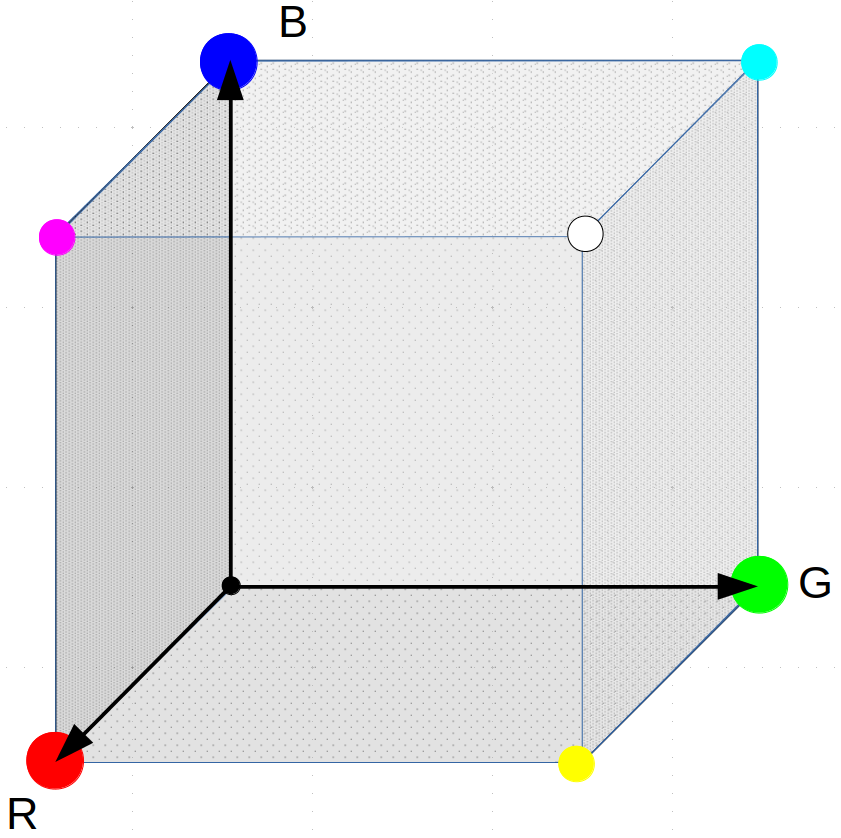
\includegraphics[scale=0.2]{Figures/CuboRGB.png}
    \caption{Espacio RGB}
    \label{fig:RGB_Space}
\end{figure}

\subsubsection{Espacio HSV}
Szeliski describe el espacio HSV, formado con los componentes Matiz (Hue, \textit{H}), Saturación, (Saturation, \textit{S}), Brillantez o Intensidad (Value \textit{V}, Brigtness \textit{B} o Intensity, \textit{I}), mencionando que es una transformación no lineal del espacio de color RGB, correspondiente de igual manera a una tercia de valores que describen el color de interés.

Sonka y Hlavac \cite{czerwinski_definitions_2013} detallan que este espacio de color separa la intensidad y el color, mientras que el matiz y la saturación corresponden a la percepción humana, haciendo muy útil esta representación para desarrollo de algoritmos de procesamiento de imagen, aclarando también que el uso de los valores en RGB puede hacer la manipulación de la imagen propensa a deformaciones de la percepción humana del color. 

Mencionan también que el espacio RGB es utilizado para almacenamiento, procesamiento, codificación o presentación de las imágenes en televisiones, a diferencia del espacio HSV, cuyas aplicaciones se encuentran más enfocadas a la percepción del color y al uso de la imagen en gráficos de computadora.

Los valores asociados a cada uno de los parámetros del espacio HSV son, como se mencionó anteriormente, transformaciones no lineales de los valores  $R,G,B$ y se pueden obtener mediante las ecuaciones de transformación siguientes\cite{burger_digital_2022}:

Siendo:

\begin{equation*}
C_{min} = min(R,G,B), \quad
C_{max} = max(R,G,B), \quad
\Delta = C_{max} - C_{min},
\end{equation*}

Entonces,

\begin{equation*}
    S = \begin{cases*}
  \frac{\Delta}{C_{max}}, & para $C_{max} > 0$.\\
  0, & otros casos,
    \end{cases*}
\end{equation*}

Con el objetivo de mantener los valores de estas transformaciones entre $[0,1]$, se divide entre el valor máximo que será posible que tenga la representación, comúnmente 255.

\begin{equation}
V = \frac{C_{max}}{255},
\end{equation}

\begin{equation*}
R^{'} = \frac{C_{max}-R}{\Delta},  \quad G^{'} = \frac{C_{max}-G}{\Delta},  \quad B^{'} = \frac{C_{max}-B}{\Delta},
\end{equation*}

Posteriormente, dependiendo de cuál de los colores en la representación RGB tuviera el valor máximo, se calcula un valor preliminar del matiz, de la siguiente forma:

\begin{equation*}
    H^{'} = \begin{cases*}
  B^{'} - G^{'}, & cuando $R = C_{max}$,\\
  R^{'} - B^{'}+2, & cuando $G = C_{max}$,\\
  G^{'} - R^{'}+4, & cuando $B = C_{max}$,
    \end{cases*}
\end{equation*}

Lo que resulta en una representación dentro del intervalo $[-1,5]$ y finalmente se obtiene la normalización dentro del intervalo $[0,1]$ como se muestra a continuación.

\begin{equation*}
    H = \frac{1}{6}\cdot\begin{cases*}
  (H^{'}+6), & cuando $H^{'}=0$,\\
  H^{'}, & otros casos,
    \end{cases*}
\end{equation*}

Finalmente, para obtener la representación de la componente H como el correspondiente a un ángulo se multiplica por 360.

\begin{equation*}
    H^{\circ} = H\cdot360
\end{equation*}

Este espacio puede ser gráficamente representado como un prisma circular invertido, donde el radio de la base representa el valor de la saturación (S), La altura del cono representa la intensidad (V), y el matiz (H) se obtiene mediante un ángulo trazado sobre la base del cilindro, comenzando con el color rojo, que se encuentra en 0 grados, el color verde en 120 grados y finalmente el color azul en 240 grados. 

\begin{figure}[H]
\centering
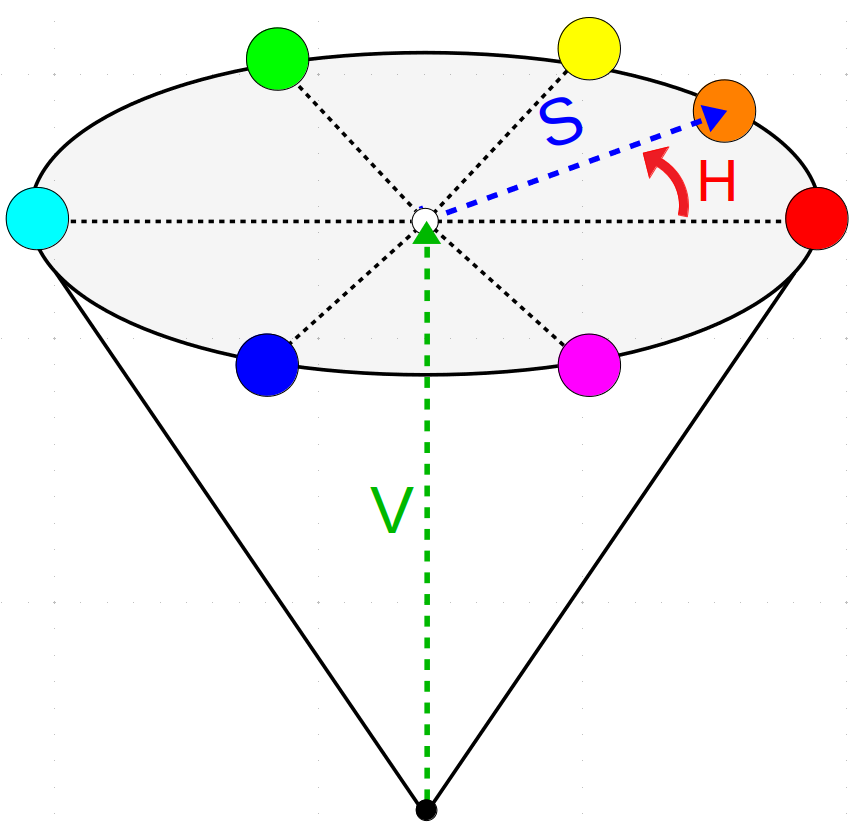
\includegraphics[scale=0.2]{Figures/ConoHSV.png}
    \caption{Espacio HSV, representación cónica}
    \label{fig:HSV_Space}
\end{figure}


\subsection{Segmentación de Imágenes}

En \cite{gonzalez_digital_2002}, los autores comentan que una segmentación robusta es un gran avance en el proceso de procesamiento de una imagen en la cual sea necesario identificar objetos. Adicionalmente, 
Sonka et al. (2018)\cite{sonka_image_2008}, ahondan en las características de la \textbf{segmentación completa} y la \textbf{segmentación parcial}. Explican que en la primera, se obtiene como resultado un conjunto de regiones no superpuestas que corresponden totalmente con \textit{objetos del mundo real} en la imagen de entrada. Mientras que en la segmentación parcial las regiones no corresponden directamente con \textit{objetos del mundo real} presentes en la imagen, sino que aíslan características específicas de la imagen, como la brillantez, el color, la textura, etc. Dada la complejidad asociada a la segmentación completa de las imágenes, para obtenerlas es necesario aplicar niveles más altos de procesamiento a comparación de la segmentación parcial.



Se dice que la segmentación completa de una imagen R es el conjunto finito de regiones $R_{1}, ..., R_{S}$, expresado matemáticamente como: 

\begin{equation*}
R = \bigcup^{S}_{i = 1}, \quad
R_{i} \cap R_{j} = 0, \quad
i \neq j
\end{equation*}

\subsubsection{Umbralización}
La umbralización es una de las herramientas más antiguas para realizar segmentación de imágenes, y tiene como ventaja que no requiere muchos recursos computacionales para realizarla, por lo que es todavía ampliamente utilizada en diferentes aplicaciones. Esta técnica consiste en establecer valores dentro de los cuales se considera aceptable la característica de interés.

Este proceso corresponde a la transformación de una imagen de entrada $f$ a una salida segmentada, una imagen binaria $g$, de la siguiente forma:

\begin{equation*}
g(i,j) =\begin{cases*}
1, & para $f(i,j) \geq T$,\\
0, & para $f(i,j) < T$ \end{cases*} 
\end{equation*}
\phantom{saltodelinea}\\

Donde $T$ representa el umbral (Threshold). Después de esta trasnformación, todos los pixeles dentro de la imagen que se encuentren dentro del/los umbrales definidos tendrán un valor de 1 y a aquellos que no satisfagan la condición se les asigna el valor 0 (o vice versa) \cite{sonka_image_2008}. \phantom{saltodelinea}



González y Woods \cite{gonzalez_digital_2002} describen el proceso de segmentación de imágenes en el espacio HSV de la siguiente manera:
\begin{itemize}
    \item Separar la imagen en sus componentes HSV.
    \item Reconocer las zonas de la imagen (y los valores de los píxeles) donde se encuentran las características de interés.
    \item Establecer los umbrales de los valores HSV que determinan los píxeles que representan la información de valor.
    \item Umbralizar: generar una máscara binaria con las regiones donde se encuentran dichos valores.
    \item Utilizar la máscara y la imagen original para aislar las regiones de interés de la imagen.
\end{itemize}


\subsection{Operaciones Morfológicas}

González y Wood explican también que bajo el contexto de procesamiento de imágenes la \textit{morfología matemática} hace alusión a una herramienta para extraer los componentes de la imagen que son útiles para la representación y descripción de la forma de una región. Indica además que el lenguaje que se ha de utilizar para este procesamiento es la teoría de conjuntos y resaltan que los conjuntos en \textit{morfología matemática} representan objetos en una imagen.
Debido a la relación mencionada entre el procesamiento morfológico de la imagen y la teoría de conjuntos, se explican en enseguida algunos conceptos iniciales.

\subsubsection{Teoría de Conjuntos}
Sea $A$ un conjunto perteneciente a $Z^2$. Si $a = (a_{1}, a_{2})$ es un elemento de $A$, se representa de la siguiente forma: $a \in A$. De forma similar, si $a$ no es un elemento de $A$, se representa como: $a\notin A$.

Aquel conjunto en el cual no hay elementos se conoce comúnmente como el conjunto \textit{nulo} o conjunto \textit{vacío} y se utiliza el símbolo $\oslash$.

Un \textbf{conjunto} se representa por lo contenido entre dos llaves: $\{\cdot\}$ y los elementos de los conjuntos que son de nuestro interés en este contexto son los píxeles que componen una imagen digital.

Si todos los elementos de A se encuentran también en el conjunto B, se dice que el conjunto A es un \textbf{subconjunto} del B y se escribe de la siguiente forma:

\begin{equation*}
A\subseteq B
\end{equation*}

La \textbf{unión} $C$ de los conjuntos $A$ y $B$ es aquel conjunto al que pertenecen todos los elementos ya sea de A, B o de ambos y se expresa como:

\begin{equation*}
C = A \cup B
\end{equation*}

La \textbf{intersección} $D$ de dos conjuntos es el conjunto que contiene a los elementos que pertenecen a $A$ y a $B$:

\begin{equation*}
D = A \cap B
\end{equation*}

\begin{figure}[H]
\centering
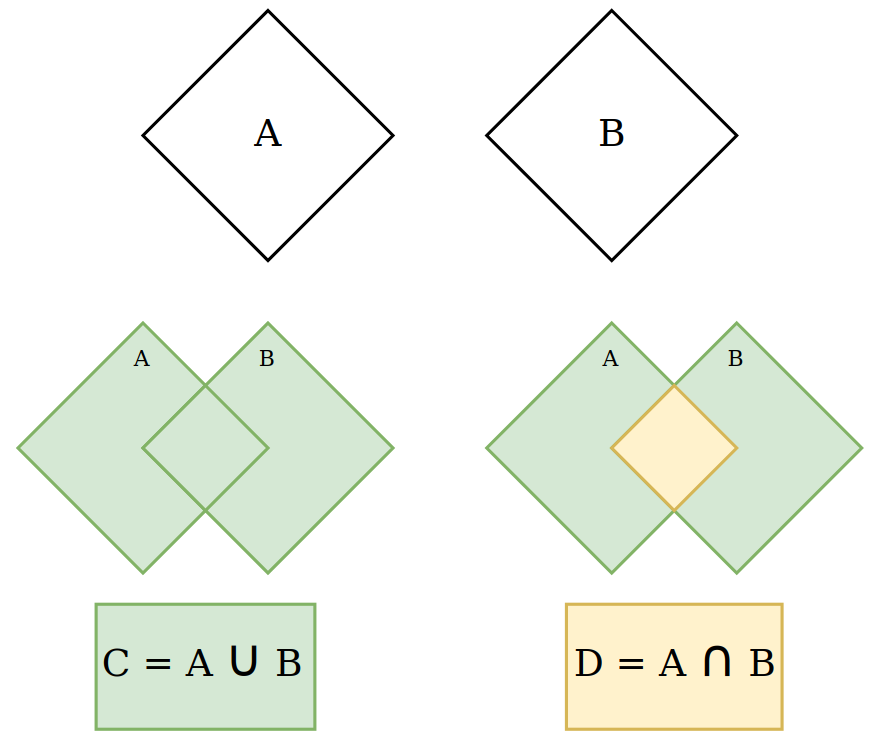
\includegraphics[scale=0.3]{Figures/Conjuntos.png}
    \caption{Unión e Intersección de Conjuntos}
    \label{fig:UnioneInterseccion}
\end{figure}

Se dice que dos conjuntos son \textbf{mutuamente excluyentes} si no tienen ningún elemento en común, 

\begin{equation*}
A \cap B = \oslash
\end{equation*}

El \textbf{complemento} del conjunto A es el conjunto de todos aquellos elementos que no pertenecen a A.

\begin{equation*}
A^{C} = \{\omega \mid \omega \notin A\}
\end{equation*}
Dado el conjunto Universal $U$:
\begin{figure}[H]
\centering
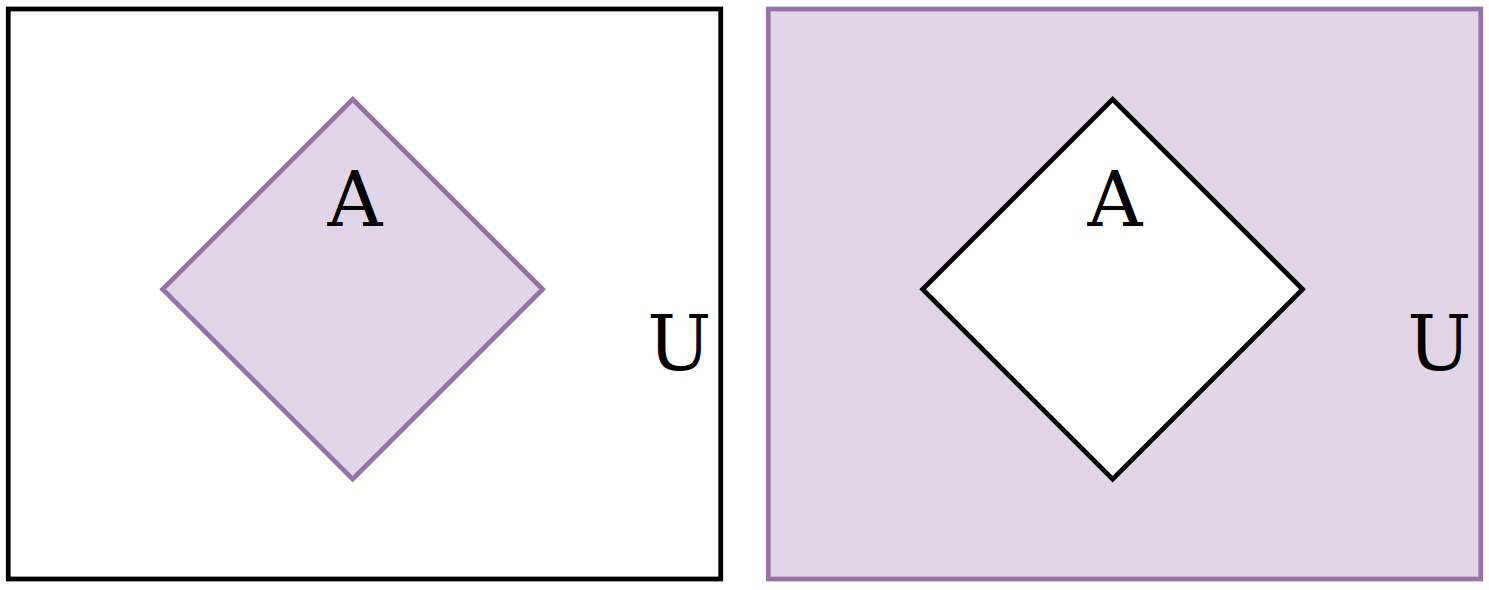
\includegraphics[scale=0.17]{Figures/Conjuntos_Complemento.png}
    \caption{Complemento}
    \label{fig:Complemento}
\end{figure}

La \textbf{diferencia} entre dos conjuntos $A$ y $B$ representada como $A-B$, es el conjunto de elementos que pertenecen a A pero no a B se define como:

\begin{equation*}
A - B = \{ \omega \mid \omega \in A, \omega \notin B \} = A \cap B^{C}
\end{equation*}

\begin{figure}[H]
\centering
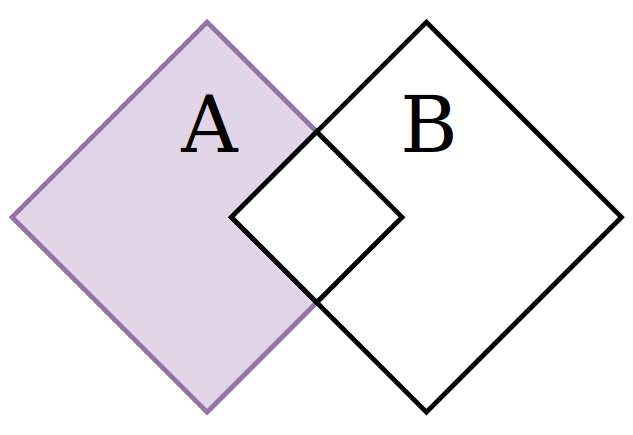
\includegraphics[scale=0.17]{Figures/Conjuntos_Resta.png}
    \caption{Diferencia}
    \label{fig:Diferencia}
\end{figure}

La reflexión del conjunto B se define como:

\begin{equation*}
\hat{B} = \{ \omega \mid \omega -b, \textup{ para } b \in B \}
\end{equation*}

\begin{figure}[H]
\centering
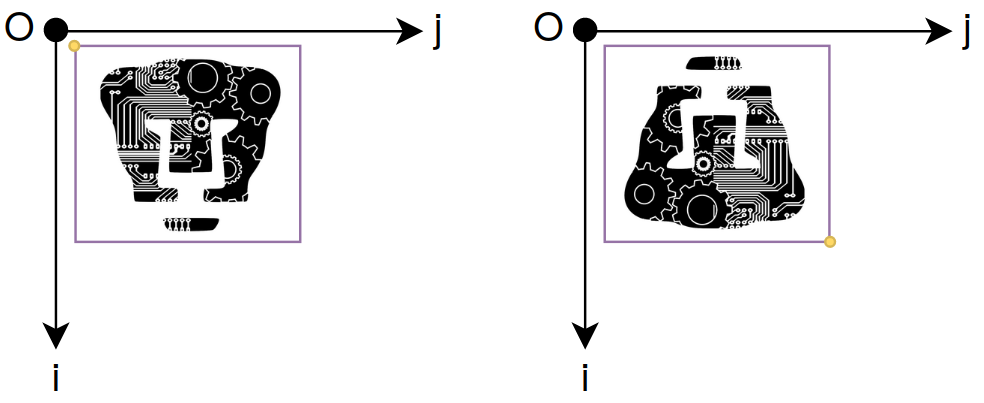
\includegraphics[scale=0.32]{Figures/Reflexion.png}
    \caption{Reflexión}
    \label{fig:Reflexion}
\end{figure}

La traslación del conjunto A al punto $Z = (z_{1}, z_{2})$, representada como $(A)_{z}$, se define como:

\begin{equation*}
(A)_{z} = \{ c \mid c = a+z, \textup{ para } a \in A \}
\end{equation*}

\begin{figure}[H]
\centering
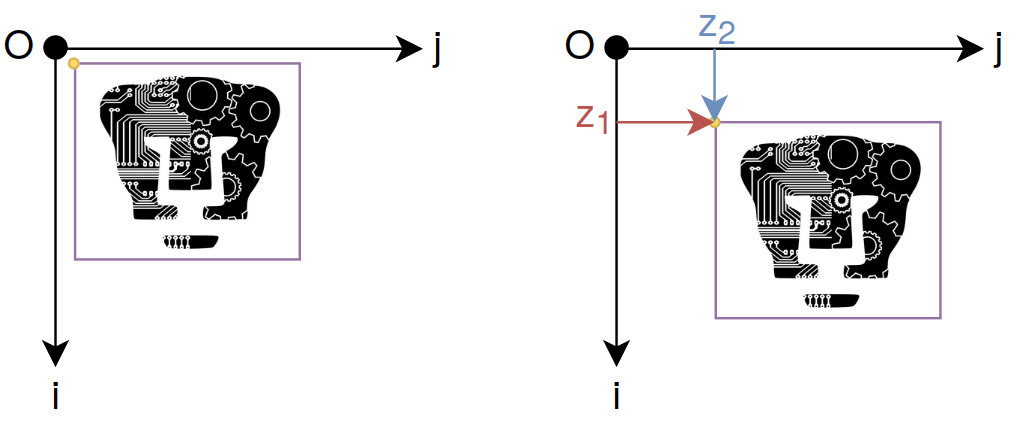
\includegraphics[scale=0.32]{Figures/Traslacion.png}
    \caption{Traslación}
    \label{fig:Traslacion}
\end{figure}

En las figuras \ref{fig:Reflexion} y \ref{fig:Traslacion} el origen de las imágenes originales se encuentra resaltado con un punto amarillo.

\subsubsection{Operaciones Lógicas}

Comúnmente el procesamiento morfológico se realiza sobre imágenes en blanco y negro, es decir, imágenes en donde los únicos valores posible para los píxeles son 1 y 0, esto permite que se utilicen operaciones binarias sobre los píxeles de la imagen. 
Algunas de las operaciones binarias que con más frecuencia se utilizan para el procesamiento de imágenes son las operaciones \textbf{AND}, \textbf{OR}, y \textbf{NOT}. Las dos primeras permiten operar entre dos o más imágenes, como en el caso de aplicar una máscara sobre una imagen, utilizando la operación AND. En la Figura \ref{fig:LogicOp} se muestra el comportamiento de estas operaciones lógicas.

\begin{figure}[H]
\centering
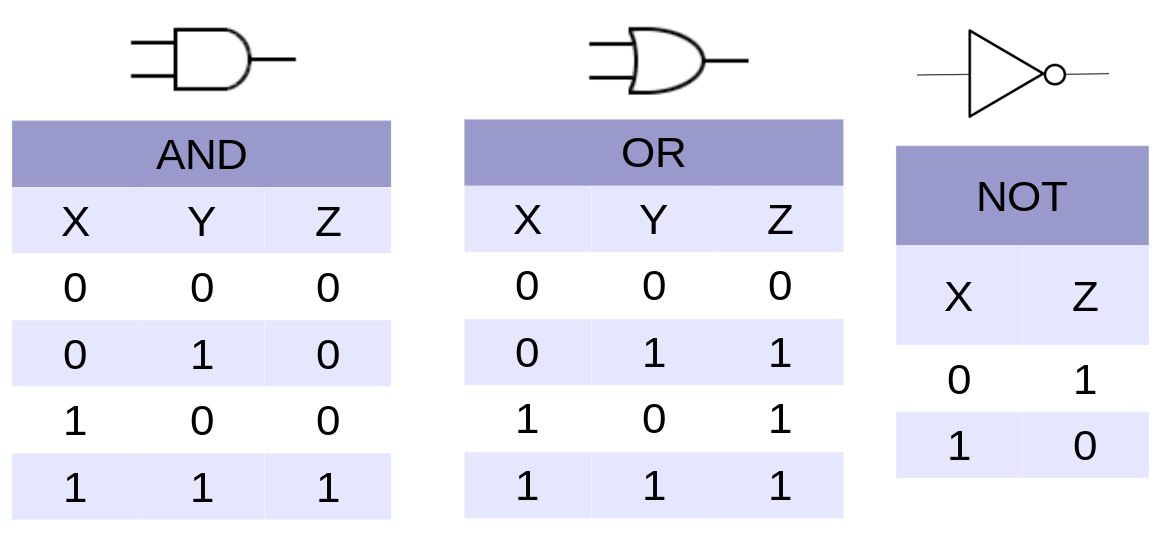
\includegraphics[scale=0.2]{Figures/CompuertasLogicas.png}
    \caption{Operaciones Lógicas AND, OR y NOT}
    \label{fig:LogicOp}
\end{figure}

Estas operaciones tienen comportamientos similares a los mencionados en teoría de conjuntos, con la limitante de que las operaciones lógicas solo pueden ser utilizadas con valores binarios después de la umbralización de los valores de los píxeles de la imagen, en la Figura \ref{fig:LogicOpIMG} se observa un ejemplo del comportamiento de estas operaciones en una imagen binaria.
\begin{figure}[H]
\centering
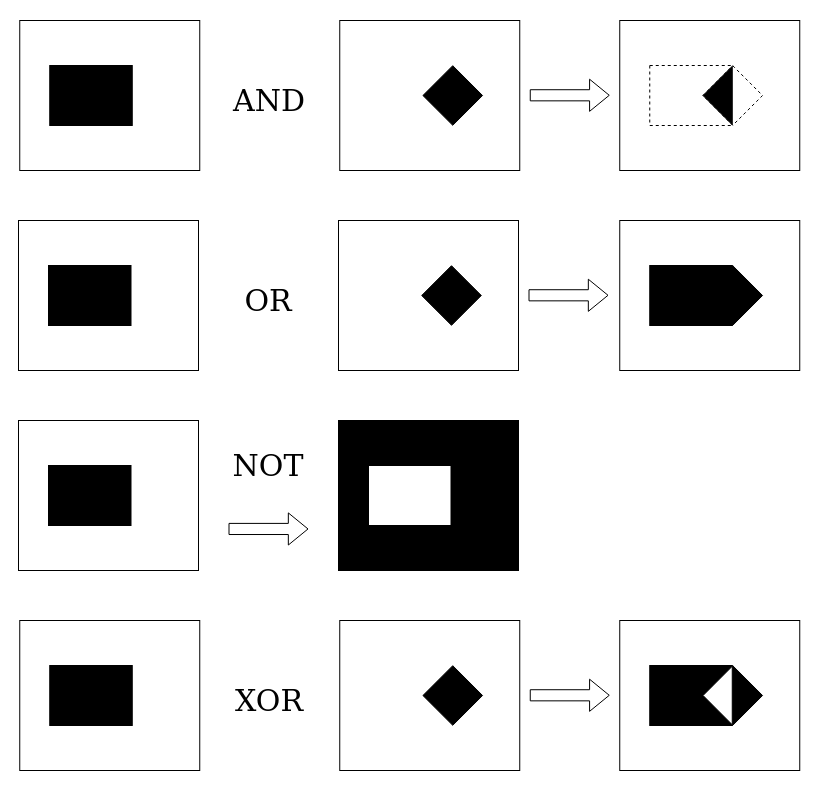
\includegraphics[scale=0.3]{Figures/LogicOp_IMG.png}
    \caption{Operaciones Lógicas Aplicadas a Imagen}
    \label{fig:LogicOpIMG}
\end{figure}

\subsubsection{Dilatación y Erosión}

Estas operaciones se consideran básicas dentro el procesamiento morfológico de las imágenes y algunas  de las técnicas más avanzadas que se utilizan, se basan en ellas.

\emph{Dilatación}\\
Siendo $A$ y $B$ dos conjuntos en $Z^2$, la dilatación de $A$ y $B$, expresada como $A \oplus B$, se define como:

\begin{equation*}
A \oplus B = \{ z \mid (\hat{B})_{Z} \cap A \neq \oslash \}
\end{equation*}

Para obtener esta ecuación es necesario obtener la reflexión de $B$ sobre su origen e invirtiendo su reflexión en $z$. La dilatación de A por B es el conjunto de todos los desplazamientos de $z$, tal que B y A se sobreponen por al menos un elemento. De acuerdo con esta descripción, es posible re-escribir la anterior definición como:

\begin{equation*}
A \oplus B = \{ z \mid [(\hat{B})_{Z} \cap A] \subseteq A \}
\end{equation*}

en estas ecuaciones, el conjunto $B$ es comúnmente mencionado como el \textit{elemento estructurante} de la dilatación y otras operaciones.

Vale la pena mencionar que esta definición de la operación dilatación coincide con el proceso para realizar la convolución, dado que de forma similar se \textit{invierte} uno de los operandos y se recorre sobre el otro elemento de la operación. Es importante recalcar que la convolución es una más de las operaciones que con frecuencia se utilizan para el procesamiento de imágenes, por ejemplo para el filtrado de las imágenes, al hacer la convolución de la forma matricial de la imagen con la matriz que represente el filtro que se busca aplicar. 

\emph{Erosión}


Para los conjuntos $A$ y $B$, pertenecientes a $Z^{2}$, la operación erosión, representada como $A \ominus B$, se define como:

\begin{equation*}
A \ominus B = \{ z \mid (B)_{Z} \subseteq A \}
\end{equation*}

Es decir, la erosión aplicada a estos conjuntos resulta en el conjunto de todos los puntos $z$, tal que B (traducido en puntos $z$), que son contenidos en A.

En la figura \ref{fig:Ero+Dil} se muestra un ejemplo de los efectos de la operación morfológica, a)Imagen original, b)Matriz de 3x3 como Elemento estructurante, c)Operación Erosión aplicada a la Imagen Original, d)Operación Dilatación aplicada a c).

\begin{figure}[H]
\centering
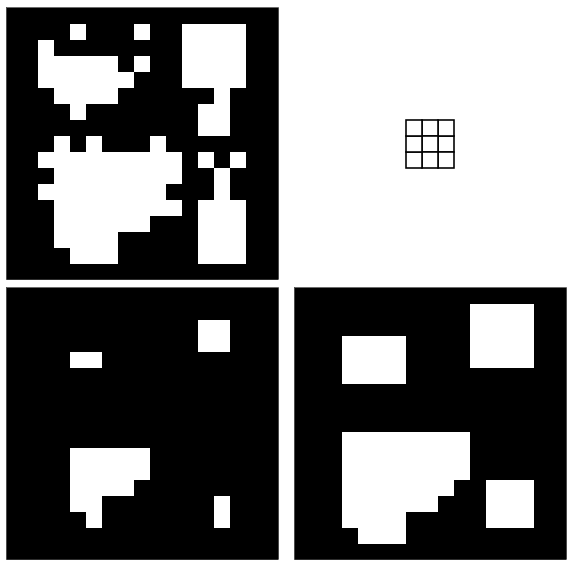
\includegraphics[scale=0.53]{Figures/ErosDil_NoGrid.png}
    \caption{Operaciones Morfológicas: Dilatación y Erosión}
    \label{fig:Ero+Dil}
\end{figure}

Como es posible notar en el ejemplo, estas dos operaciones no son estrictamente inversas entre sí. Además, dado que al realizar la operación erosión se pierde información sobre los detalles de la imagen original, es imposible recuperarla aplicando la dilatación. Adicionalmente, elemento estructurante tiene gran influencia en el resultado que se obtendrá, dado que una modificación en sus dimensiones o su forma resulta en una evidente modificación de la imagen final, un ejemplo de esto puede verse en la figura \ref{fig:Dil_ES2}, utilizando nuevamente  \ref{fig:Ero+Dil}, inciso c) como imagen base.

\begin{figure}[H]
\centering
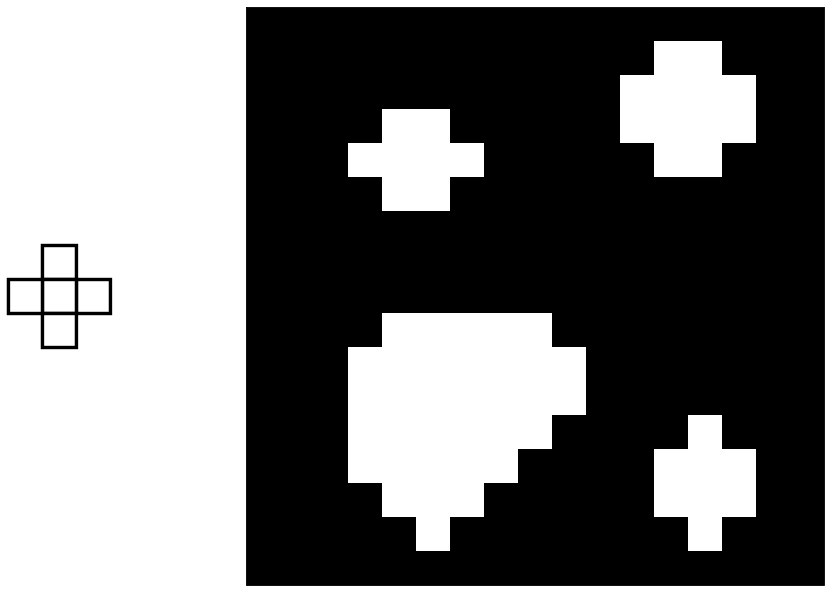
\includegraphics[scale=0.25]{Figures/Dil_ES2.png}
    \caption{Dilatación aplicada con distinto Elemento Estructurante}
    \label{fig:Dil_ES2}
\end{figure}

%%Detección de Bordes y Filtro Gaussiano

\section{Reconocimiento de Objetos}
Una de las partes fundamentales de la visión computacional es la habilidad de reconocer objetos dentro de las imágenes que son procesadas, para lo cual se utilizan algoritmos de reconocimiento de patrones que nos permiten clasificar objetos o regiones dentro de la imagen, haciendo posible entender mejor los elementos que la componen.

Como se ha mencionado anteriormente, para nosotros las tareas asociadas a la visión son actividades que llevamos a cabo de manera natural, sin que requiera un esfuerzo consciente en la mayoría de los casos y, teniendo ya sea un ejemplo visual o bien una descripción sobre las características de nuestro objeto de interés, somos capaces de identificarlo dentro del entorno. Con el objetivo de reconocer los objetos mediante el análisis computacional de las imágenes, es imprescindible conocer las características de dichos objetos, así como de las clases a las que pertenecen.

De acuerdo con Sonka \cite{sonka_image_2008}, el diseño de una adecuada representación del conocimiento es la parte más importante de la resolución del problema del entendimiento y se refieren a las descripciones y las características como una representación de \textit{bajo nivel}, aclarando que no pueden ser consideradas en sí mismas como representaciones del conocimiento, aunque sí pueden ser usadas como parte de una estructura de representación más compleja.

Se ha dicho antes que como humanos podemos utilizar descripciones verbales o escritas de la apariencia de un objeto y utilizar esa información para identificarlos, sin embargo, para que una máquina pueda replicar este comportamiento es necesario tener  una representación de esta descripción que sea posible procesar matemáticamente. En este contexto las representaciones se hacen de forma numérica, asociando cada característica a una magnitud escalar. 
Para poder hacer la clasificación de objetos complejos es preferible que la descripción incluya la representación de varias propiedades del objeto en cuestión. Al conjunto de características representadas numéricamente se le conoce como \textbf{vectores de características}, que se utilizan como entradas para los algoritmos de reconocimiento. A este vector de características se le conoce también como \textbf{patrón}.

En el reconocimiento se les asignan clases a los objetos. En este proceso, el número de clases existentes es frecuentemente conocido desde el planteamiento del problema. Dependiendo del conjunto de las características de la clase que las propiedades del objeto satisfacen, se asignan a una u otra; el elemento encargado de esta la tarea de clasificación es conocido como \textbf{clasificador}.

El proceso principal para el reconocimiento de patrones se muestra en la figura \ref{fig:Pat_Recog}, donde podemos ver que un objeto es la entrada de un bloque de procesamiento del cual se obtiene el \textbf{patrón} del objeto, es decir, se construye el \textbf{vector de características} al aislar y cuantificar las propiedades del objeto. Este vector es posteriormente ingresado al clasificador y como salida del proceso se obtiene la clase a la que el objeto pertenece.

\begin{figure}[H]
\centering
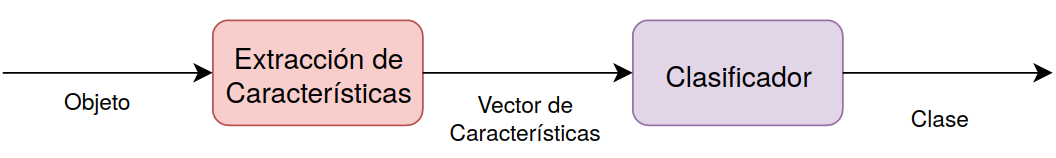
\includegraphics[scale=0.3]{Figures/Clasificacion.png}
    \caption{Reconocimiento de Objetos}
    \label{fig:Pat_Recog}
\end{figure}

Dependiendo de la aplicación para la cual se busque realizar el reconocimiento serán importantes diferentes características de los objetos. Además, las características de los recursos disponibles también encontrarán cambios. Debido a esto, se han desarrollado muchas y muy variadas técnicas de reconocimiento, utilizando cada vez diferentes características y técnicas de procesamiento de la información.
Treiber \cite{treiber_introduction_2010} en 2010, menciona que bajo los siguientes parámetros es posible definir una clasificación de los métodos de reconocimiento de objetos:

\begin{itemize}
    \item Representación de objetos: basados en la geometría (silueta, forma) o la apariencia (regiones de imagen que pertenecen al objeto).
    \item Alcance de la información sobre los objetos: características locales (descripción de una parte del objeto) o globales (información sobre el área, perímetro, etc).
    \item Variación esperada de los objetos: qué tan diferentes pueden ser los objetos dentro de una misma clase.
    \item Calidad de los datos de la imagen: dependiendo de la aplicación es posible que las imágenes a procesar contengan ruido, oclusiones o menor definición, por lo que requieren más procesamiento.
    \item Estrategia de comparación: en el proceso de reconocimiento es necesario un paso en el cual se realiza una comparación entre la similitud entre la imagen analizada y la referencia. Dependiendo del algoritmo de comparación usado cambian también los parámetros requeridos.
    \item Alcance de la información de los elementos utilizados en la comparación: el autor propone una división en las siguientes tres categorías: valores sin procesar de los píxeles de intensidad, características de bajo nivel (bordes) y alto nivel (líneas o arcos). 
\end{itemize}

Una vez establecidas estas condiciones, el autor lista algunos métodos de reconocimiento de objetos:

\begin{itemize}
    \item \textbf{Métodos globales}\\ Buscan modelar y encontrar los objetos únicamente con características globales.
    \item \textbf{Métodos basados en Transformación y Búsqueda}\\ La pose del objeto se determina buscando el espacio de transformaciones entre el modelo y la información de la imagen
    \item \textbf{Métodos basados en Correspondencia Geométrica}\\ Utilizan las relaciones geométricas entre varias parte del objeto y establece correspondencias entre el modelo y las características de la imagen.
    \item \textbf{Métodos basados en descriptores}\\ Buscan identificar los objetos utilizando descriptores, normalmente de la apariencia de los objetos en regiones locales cerca de los puntos de interés. 
\end{itemize}

El proceso utilizado en este proyecto corresponde a la última categoría de las anteriores,y fue elegido dado que su implementación no requiere muchos recursos computacionales y es suficientemente rápido para la aplicación propuesta. Además, claro, que las características de los objetos de interés lo permiten.


\section{Máquinas de Estado}

Cuando se habla de máquinas de estados nos referimos a un modelo computacional con el cual se representan procesos de lógica secuencial. En este modelo cuenta con conjuntos de entradas, salidas y el funcionamiento del sistema se compone por estados y funciones de transformación. En este modelo se establece que en cualquier momento de la ejecución es posible estar en uno y solo un estado a la vez, y el salto entre estados se condiciona por medio de las ya mencionadas funciones de transformación, que determinan si se realiza el cambio a otro de los estados.

Czerwinski y Kania \cite{czerwinski_definitions_2013}, enuncian la definición matemática de la Máquina de Estados Finitos (FSM) utilizando un vector de 5 elementos, $\{X,Y,S,\delta,\lambda\}$, donde $X$ corresponde a un espacio de entradas finitas, $Y$ al espacio de salidas finitas, $S$ a un conjunto de estados finitos, $\delta$ representa la función de transformación y $\lambda$ la función de salidas. En este caso, la función de transición de una Máquina de estados finitos determina el siguiente estado ($S^+$), y se refiere al mapeo $\delta: X \times S \to S $.


Dentro de las máquinas de estados finitas se encuentran dos grandes clasificaciones, las máquinas Moore y las máquinas Mealy, que reciben su nombre de los investigadores Eduard F. Moore y George H. Mealy, que desarrollaron \textit{la teoría del autómata}. En el planteamiento de la máquina de Moore las salidas dependen únicamente del estado actual de la máquina, expresando este comportamiento en términos de los vectores definidos anteriormente se obtiene: $\lambda: S \to Y$. Por el contrario, en las máquinas Mealy las salidas dependen tanto del estado actual como de las entradas actuales del sistema. Así, la función de salida se puede representar como: $\lambda: X \times S \to Y$.


\section{Sistemas expertos}
 
A mediados del Siglo XX, cuando el concepto de Inteligencia Artificial comenzaba a popularizarse, su aplicación principal se centraba en planeación y solución de problemas. En aquel momento era difícil imaginar que décadas más tarde las aplicaciones más importantes se encontraran en ingeniería del conocimiento y en sistemas expertos. En 1982 el profesor Edward Feigenbaum de la Universidad de Stanford, uno de los pioneros en el desarrollo de tecnología de sistemas expertos, definió un sistema experto como "un programa computacional que utiliza procedimientos de inferencia para resolver problemas que son suficientemente complicados para requerir conocimiento humano especializado para su solución."
\cite{giarratano_zhuan_2002}

En 2020, 38 años más tarde de esta definición, Gupta \cite{gupta_artificial_2020} refiere que un sistema experto es un programa computacional que emula la capacidad de razonar y el comportamiento de un humano con el conocimiento y experiencia de un experto en un campo específico. También indica que los sistemas expertos son utilizados para resolver problemas complejos utilizando el conocimiento almacenado en una base de datos en forma de reglas. 

De acuerdo con Liebowitz \cite{liebowitz_handbook_2019} la adquisición de conocimiento es el proceso de extraer, estructurar y organizar el conocimiento de diferentes fuentes, usualmente humanos expertos en un área, de forma tal que la habilidad de solucionar problemas pueda ser capturada y transformada para que una computadora sea capaz de leerla. De acuerdo con este autor: "Sin conocimiento explícitamente representado, un sistema experto no es más que un programa de computadora."

Gupta y Liebowitz señalan también que uno de los pasos intermedios entre la adquisición de conocimiento y la implementación de sistemas expertos es la intervención de un Ingeniero de conocimiento, un individuo que estudia la forma en que los expertos toman decisiones y lo traduce a reglas en términos comprensibles para la máquina. A partir de esto, Gupta menciona que los sistemas expertos son también conocidos como sistemas basados en conocimiento o sistemas expertos basados en conocimientos, así como sistemas basados en reglas, y que se consideran como Inteligencia Artificial Aplicada. 

\section{Manipulación del Robot}
Siendo la manipulación de objetos un de los objetivos principales de este proyecto es pertinente explicar la forma en que le es posible al robot tomar los objetos que se espera que transporte. Para esto, es necesario realizar el análisis cinemático del robot, que consiste en el estudio de la relación que guarda el efector final respecto a la estructura que compone el manipulador del robot, es decir el comportamiento que debe tener cada articulación del robot para que el efector final pueda posicionarse en las coordenadas finales deseadas para el comportamiento esperado del robot.

Para realizar este análisis es necesario conocer el número de grados de libertad con los que cuenta el manipulador que se usará, así como el tipo de articulaciones con las que cuenta, los ejes en los que actúa cada una y sus limitaciones de movimiento.

Ceccareli \cite{ceccarelli_fundamentals_2022}, explica que es posible formular numéricamente esta situación para determinar las coordenadas de las articulaciones $q_{i}(i=1,...,N)$ como funciones de la configuración del manipulador. Amplía diciendo que la formulación debe considerar aspectos numéricos que están relacionados a la existencia de soluciones  y a la multiplicidad de soluciones.

Los autores describen que la existencia de soluciones hace referencia a que cuando una configuración dada no se encuentre dentro del rango de movilidad del manipulador, la solución numérica de la cinemática inversa no puede ser obtenida dentro del espacio de trabajo del manipulador. Para lo cual se requiere conocer el rango de movilidad de las articulaciones y los límites del espacio de trabajo antes de unir la solución numérica. En términos matemáticos, el cumplimiento de los límites del espacio de trabajo significa que las soluciones que se obtengan pertenezcan al dominio de los números reales.

De forma similar, es posible encontrar múltiples soluciones  debido a la naturaleza \textit{altamente no lineal} de la posición cinemática de los manipuladores, es decir las diferentes configuraciones en las que se pueden posicionar los actuadores para que el efector final llegue a una coordenada determinada dentro del espacio de trabajo. 

\section{Estado del Arte}

Durante el desarrollo de este proyecto fue notable que dentro del entorno en que se plantea su desarrollo, los equipos que previamente han participado proceden sin utilizar procesamiento de imágenes en gran medida, usando en su mayoría sensores de proximidad y similares. Si bien las piezas que se tiene como objetivo que el robot identifique y sujete cuentan con características similares en forma, el color es una de las diferencias más evidentes tanto entre ellas como en relación al ambiente en que se encuentran de forma regular y se considera una característica de mucha utilidad en detección de objetos. Aunque es cierto que el entorno de la competencia en que se plantea la evaluación del comportamiento de este desarrollo se encuentra bajo condiciones controladas y es evidentemente una simulación de las condiciones de ejecución reales de un ambiente industrial, se sigue considerando conveniente el uso de cámaras y procesamiento de imágenes que permitan explotar la mayor cantidad de recursos disponibles, además de que este enfoque ofrece un aumento en la vesatilidad de la información recabada sobre el desempeño de lo sistemas.

\subsection{Antecedentes en RoboCup Logistics}
Dentro de la documentación disponible en el sitio web oficial de la RoboCup se listan los \textit{Team Description Paper} (TDP), donde se describen las técnicas utilizadas en la competencia por los equipos participantes. En estos documentos se encuentran pocos referentes de cámaras utilizadas en secciones de la competencia fuera de la localización de los códigos ARUCO en las estaciones. Estas cámaras se encuentran típicamente en la parte inferior de los robots. En el TDP presentado por el equipo austriaco GRIPS (Graz Robust and Intelligent Production System) para su participación en la competencia del 2021 \cite{furbaß_robocup_2021}, el equipo describe que, para la alineación con la banda transportadora, el robot inicia en una posición de referencia cercana a la estación, desde la cual se utiliza el sensor láser y el código ARUCO que se encuentra en sus paredes para realizar la alineación. El equipo reconoce que este primer alineamiento, combinando la información de estas dos fuentes, no es muy preciso. Por lo anterior, utilizan una segunda cámara que se encuentra en una posición más elevada para los movimientos más finos del proceso. 

\begin{figure}[H]
    \centering
    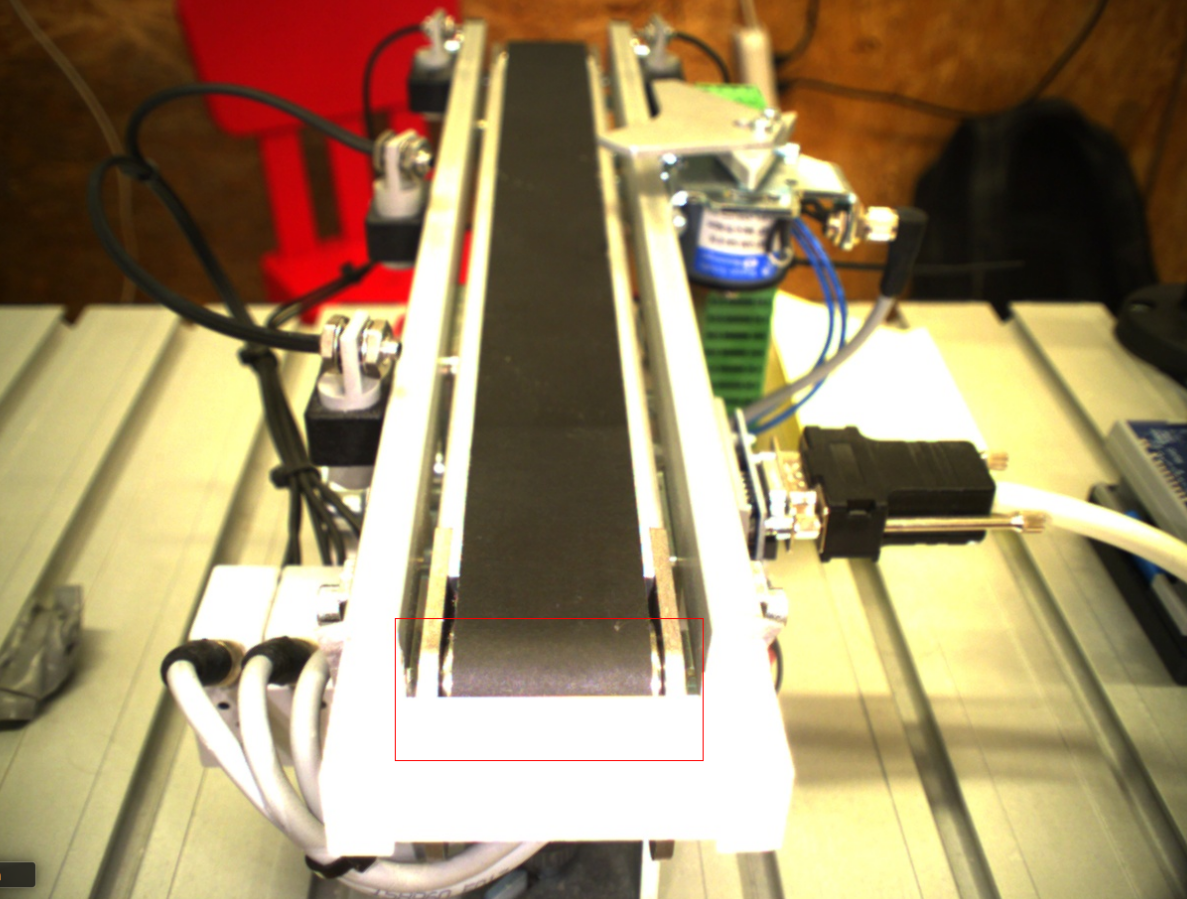
\includegraphics[scale=0.15]{Figures/Conveyor_GRIPS_TDP.png}     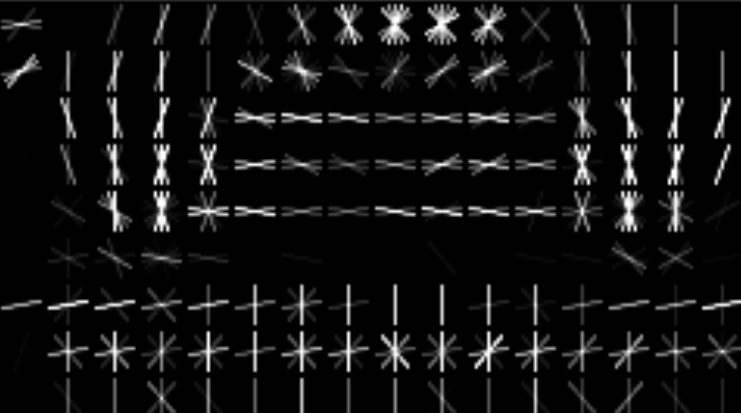
\includegraphics[scale=0.2]{Figures/Conveyor_HOG_GRIPS_TDP.png}
        \caption{Detección de Histogramas de Gradientes Orientados \cite{furbaß_robocup_2021}}
        \label{fig:HOG_GRIPS}
    \end{figure}

Con este objetivo implementaron un detector de Histogramas de Gradientes Orientados (HOG, por sus siglas en inglés). con el cual detectan la posición de los diferentes elementos de interés dentro del espacio de trabajo. Los autores describen que el HOG identifica regiones de la imagen, en las cuales se encuentran las características más representativas de los elementos ambientales. Para este punto del proceso, las características mencionadas ya eran conocidas por el algoritmo, para lo cual fue necesaria la toma de imágenes de entrenamiento y evaluación. Una vez que se aisla la zona de interés, el HOG genera un conjunto de características. Los autores mencionan que las imágenes de entrenamiento se utilizan para encontrar las características que describen las regiones de interés y las imágenes de evaluación para verificar que dichas características realmente coincidan con los objetos, como es típico en procesos de este tipo.

La descripción del proceso provista por los autores especifica que, una vez que el robot se encuentra en la posición adecuada, la cámara superior toma 4 imágenes con diferentes iluminaciones, logrados con fuentes de luz con las que cuenta el robot. Este esfuerzo se realiza con el objetivo de mitigar los errores debidos a las variaciones de iluminación naturales, y promover una correcta detección de las características de interés aún si las condiciones en las que se encuentra la estación no corresponden con las imágenes con las que fue previamente entrenado el algoritmo. Adicionalmente, para intentar robustecer el procedimiento, los autores utilizaron varios HOG en diferentes objetos, entrenando cada uno con diferentes conjuntos de imágenes, buscando diversificar las características de entrenamiento para su algoritmo de reconocimiento. En la figura \ref{fig:Robotino_GRIPS} se observan las modificaciones que el equipo GRIPS llevó a cabo en su robot hasta la edición 2021 de la competencia. Sin embargo, actualmente la implementación ya no cuenta con la cámara elevada y la estructura superior ha sido descartada.

\begin{figure}[H]
    \centering
    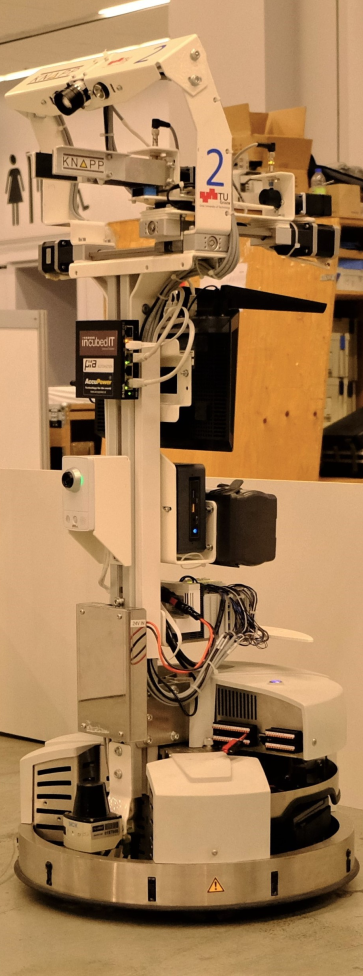
\includegraphics[scale=0.25]{Figures/RobotinoGRIPS_Old.png}
        \caption{Robotino modificado - GRIPS \cite{furbaß_robocup_2021}}
        \label{fig:Robotino_GRIPS}
\end{figure}

Para realizar la tarea de alineación, el equipo utiliza una combinación de sensores de proximidad que se encuentran debajo de y en el centro de la pinza del manipulador, utilizando también un movimiento que combina la alineación del robot con la máquina y del manipulador con la banda transportadora.

De manera similar, dentro del desarrollo del trabajo para la siguiente participación en la competencia, se planea integrar sensores de proximidad, combinando los avances obtenidos del presente proyecto, con las herramientas vistas durante lo experimentado en la edición 2023. Cabe mencionar que la configuración mecánica de los manipuladores de ambos equipos es y seguirá siendo distinta. 

\subsection{Segmentación por Color}
Debido a su bajo costo de procesamiento los algoritmos de segmentación de imágenes por color siguen siendo utilizados constantemente en gran variedad de aplicaciones. Una de ellas, es la detección de enfermedades en plantas dentro de la industria agrícola. En 2022, Hassan et.al. \cite{HASAN20227212} 


